% Options for packages loaded elsewhere
\PassOptionsToPackage{unicode}{hyperref}
\PassOptionsToPackage{hyphens}{url}
\documentclass[
  11pt,
]{article}
\usepackage{xcolor}
\usepackage[margin=1.0in]{geometry}
\usepackage{amsmath,amssymb}
\setcounter{secnumdepth}{-\maxdimen} % remove section numbering
\usepackage{iftex}
\ifPDFTeX
  \usepackage[T1]{fontenc}
  \usepackage[utf8]{inputenc}
  \usepackage{textcomp} % provide euro and other symbols
\else % if luatex or xetex
  \usepackage{unicode-math} % this also loads fontspec
  \defaultfontfeatures{Scale=MatchLowercase}
  \defaultfontfeatures[\rmfamily]{Ligatures=TeX,Scale=1}
\fi
\usepackage{lmodern}
\ifPDFTeX\else
  % xetex/luatex font selection
\fi
% Use upquote if available, for straight quotes in verbatim environments
\IfFileExists{upquote.sty}{\usepackage{upquote}}{}
\IfFileExists{microtype.sty}{% use microtype if available
  \usepackage[]{microtype}
  \UseMicrotypeSet[protrusion]{basicmath} % disable protrusion for tt fonts
}{}
\makeatletter
\@ifundefined{KOMAClassName}{% if non-KOMA class
  \IfFileExists{parskip.sty}{%
    \usepackage{parskip}
  }{% else
    \setlength{\parindent}{0pt}
    \setlength{\parskip}{6pt plus 2pt minus 1pt}}
}{% if KOMA class
  \KOMAoptions{parskip=half}}
\makeatother
\usepackage{longtable,booktabs,array}
\usepackage{calc} % for calculating minipage widths
% Correct order of tables after \paragraph or \subparagraph
\usepackage{etoolbox}
\makeatletter
\patchcmd\longtable{\par}{\if@noskipsec\mbox{}\fi\par}{}{}
\makeatother
% Allow footnotes in longtable head/foot
\IfFileExists{footnotehyper.sty}{\usepackage{footnotehyper}}{\usepackage{footnote}}
\makesavenoteenv{longtable}
\usepackage{graphicx}
\makeatletter
\newsavebox\pandoc@box
\newcommand*\pandocbounded[1]{% scales image to fit in text height/width
  \sbox\pandoc@box{#1}%
  \Gscale@div\@tempa{\textheight}{\dimexpr\ht\pandoc@box+\dp\pandoc@box\relax}%
  \Gscale@div\@tempb{\linewidth}{\wd\pandoc@box}%
  \ifdim\@tempb\p@<\@tempa\p@\let\@tempa\@tempb\fi% select the smaller of both
  \ifdim\@tempa\p@<\p@\scalebox{\@tempa}{\usebox\pandoc@box}%
  \else\usebox{\pandoc@box}%
  \fi%
}
% Set default figure placement to htbp
\def\fps@figure{htbp}
\makeatother
\setlength{\emergencystretch}{3em} % prevent overfull lines
\providecommand{\tightlist}{%
  \setlength{\itemsep}{0pt}\setlength{\parskip}{0pt}}
\usepackage{helvet} % Helvetica font
\renewcommand*\familydefault{\sfdefault} % Use the sans serif version of the font
\usepackage[T1]{fontenc}

\usepackage[none]{hyphenat}

\usepackage{setspace}
\doublespacing
\setlength{\parskip}{1em}

\usepackage{lineno}

\usepackage{pdfpages}
\usepackage{bookmark}
\IfFileExists{xurl.sty}{\usepackage{xurl}}{} % add URL line breaks if available
\urlstyle{same}
\hypersetup{
  pdftitle={Spatio-temporal distinct patterns in variations of PM\_\{10\} and PM\_\{2.5\} relative to the recent drivings of emission sources in Mongolia},
  hidelinks,
  pdfcreator={LaTeX via pandoc}}

\title{\textbf{Spatio-temporal distinct patterns in variations of
\(PM_{10}\) and \(PM_{2.5}\) relative to the recent drivings of emission
sources in Mongolia}}
\author{}
\date{\vspace{-2.5em}}

\begin{document}
\maketitle

\vspace{35mm}

Running title: INSERT RUNNING TITLE HERE

\vspace{35mm}

Munkhtsetseg\^{}1\^{}5\(^*\), Shimizu. A\^{}2, Matsuki. A\^{}3, Batdorj.
D\^{}4, Matsui. H\^{}1\(^*\)

\vspace{40mm}

\(^*\) To whom correspondence should be addressed:
\href{mailto:e.munkhtsetseg@yahoo.com}{\nolinkurl{e.munkhtsetseg@yahoo.com}}

1. Nagoya University, Japan

2. NIES

\newpage
\linenumbers

\subsection{Abstract (150 words)}\label{abstract-150-words}

Storyline:

\begin{enumerate}
\def\labelenumi{\arabic{enumi}.}
\tightlist
\item
  A new pattern is emerged
\item
  Air quality in urban sites is episodically dictated by dust events in
  spring or late autumn, yet seasonally governed by anthropogenic
  emissions in winter. {[}Air quality is governed by natural dust
  emission, and anthropogenic emissions{]}
\item
  With recent growing interest in urban life style, and combustion of
  coal/oyutolgoi for heating winter conditions results a highly increase
  in not only capital city but also towns
\item
  In a result, spring coarse dust, plus winter fine pollutants
\item
  spring coarse dust is immediately transported and deposited in the
  source area, whereas winter fine pollutants is permanently stayed in
  the source area due to stagnant atmosphere govern over entire
  country., perhaps floating in the near surface, deposits in the
  surface{]}
\item
  Alarms, the Mongolian dust in the spring, optical properties might be
  shifted; this gives \ldots{} Gobi dust and sand storms has become
  tuiren, from the shoroon shuurga. which clearly requires the
  attention.
\item
  r ratio shows \ldots{} emission source; dust might carry anthropogenic
  fine particulates as well. \newpage
\end{enumerate}

\subsection{Introduction}\label{introduction}

\begin{verbatim}
* Advanced the knowledge of global dust, has reached to recognize the sources,.
  - Classification dust brown color, seasonal characteristics, with coarse fractions.
  - This knowledge further efficient to climate system when elaborating dust-aerosol effects.
  - But, a large uncertainties in the global dust model has existed so for climate models which clearly limits our understanding the climate system and shape the facing global issues of global warming.
  - This is mainly caused by the lack of parameterization and recognition of iterative changes controlled by the natural forces and anthropogenic drivings.

* Mongolian dust brown color, seasonal characteristics, with coarse fractions.
  - Mongolian dust has an attention of the its mass fraction in global dust, yet unlikely elaborated in the climate models due to its majority of coarse fraction for its a small contribution to the climate system through its radiative feedback.
  - But, such recognized characterization might get no longer valid due to recent change in the driving of the emissions of air particulate matters. A large high concentrations of PM2.5 in the capital city of Mongolia has been observed  as a result of the heavy consumptions of coal as a winter heating has rapidly spread as a mining industry taken off since 2000. Winter weather stagnant conditions governed by the Siberian magnifies the concentrations of the particulate matter emissions by trapping the polluted air below the boundary layer, so that results in a very large high concentrations of PM2.5, locally. Even  recognized as one of the highly polluted capital cities in the world.
  - Therefore, It is important to examine the emerging changes and shifting patterns of air particulate matters in Mongolia. More importantly, it is essential to reveal the significant changes in the the altered fraction particularly, in the dust seasons considering its high potential of intriuging in the free atmosphere to transported in the long-distance, so carrying capacity of the role to shift the global climate system, and its side impacts on downwind regions.
\end{verbatim}

\begin{itemize}
\tightlist
\item
  Study goal

  \begin{itemize}
  \tightlist
  \item
    We hypothesize \ldots{}
  \item
    Our study will benefit not only to the global dust research but also
    climate, and further to the country itself for urban planning, and
    coal combustion.
  \end{itemize}
\end{itemize}

\subsection{Research Qs}\label{research-qs}

Therefore, we aimed to demonstrate the distinct temporal and spatial
variations of PM2.5 and PM10 across urban and rural Mongolia using
extensive data from 2008 to 2020.

On spring, the dust storm from the Gobi Desert contribute significantly
to increased aerosols in the atmosphere and ambient air pollution,
leading to sporadic peaks in PM10 concentrations reaching as high as
64-234 \(\mu g m^{-3}\) per day or exceeding 6000 \(\mu g m^{-3}\) per
hour (Jugder). concentrations of particulate matter is ephederemal, yet
vary depending on whether the pollution cause is natural or industrial,
local or transported, seasonal or non-seasonal, makes complex and
challenging. 1. Do concentrations of particulate matters differ in
between urban and rural sites, and even within Gobi sites? 2. Do
distinct temporal variations has existed among the sites? 3. Do PM2.5
particulates has contributed to the PM10 annual variations?

\begin{verbatim}
-   If yes, how much, and when and where?
-   What is the sd, mean, and median
    -   box plot
    -   violin
    -   scatter points, epidemic, sporadic
-   Daily variations to examine it related to the heating
    -   2 peaks: smaller and bigger
    -   compare the t-duration exceeds 50mug/m3/hour

4.  Does it has distinct patterns among the sites regarding to the
    drivings

-   How PMs varies with the wind speed and visibility
-   Do they differently explained with variables and changes in
    drivings (with PCA analysis)

5.  Is there any significant changes in time-series of PMs at 4
    seasons
6.  Is there any significant changes in ratio in the spring in
    respect to winter?

    The present study will contribute significantly to the understanding
        of air particulate matter patterns in Mongolia and providing
        comprehensive data insights for policymakers and public health
        sectors. Our findings is useful not only for addressing national health
        impacts but also beneficial for understanding air particulate matter
        as ambient air pollution, and tackling atmospheric aerosol effects
        in the climate system, and revealing their transboundary effects to
        the downwind regions in South-east Asia.
\end{verbatim}

\subsection{Results}\label{results}

\subsubsection{The spatio-temporal variations of the PMs at the study
sites}\label{the-spatio-temporal-variations-of-the-pms-at-the-study-sites}

\subsection{To evaluate the spatial variations in particulate matter
(PM) concentrations, we displayed hourly observed values of PM10 and
PM2.5 for all study sites (figure\_3). The mean p-values indicate that
PM concentrations differ significantly at a 99\% confidence level across
all sites (figure\_3), with the exception of a 95\% confidence level
between DZ and UB for PM10 (figure\_3a), highlighting substantial
concentration disparities among sites. While quantitative differences in
PM concentration values exist across all sites, two key patterns emerge
when examining median deviations from mean values and irregular
observation fluctuations. For instance, PM10 demonstrates more erratic
behavior than PM2.5 at each location, particularly evident at ZU and SS
sites. Furthermore, the mean values calculated from hourly measurements
surpass the median concentrations for both PM10 and PM2.5 across all
sites, with notable prominence at UB and DZ locations. Consequently,
significant spatial differences in PM concentrations exist among all
sites, regardless of urban or rural classification. However, the sites
can be categorized into two groups based on their characteristics: UB
(urban) and DZ (rural town, Gobi); and SS (rural, Gobi) and ZU (rural,
Gobi). These findings for DZ appear to support our hypothesis of
emerging new emission patterns related to increased coal consumption
during winter
months.}\label{to-evaluate-the-spatial-variations-in-particulate-matter-pm-concentrations-we-displayed-hourly-observed-values-of-pm10-and-pm2.5-for-all-study-sites-figure_3.-the-mean-p-values-indicate-that-pm-concentrations-differ-significantly-at-a-99-confidence-level-across-all-sites-figure_3-with-the-exception-of-a-95-confidence-level-between-dz-and-ub-for-pm10-figure_3a-highlighting-substantial-concentration-disparities-among-sites.-while-quantitative-differences-in-pm-concentration-values-exist-across-all-sites-two-key-patterns-emerge-when-examining-median-deviations-from-mean-values-and-irregular-observation-fluctuations.-for-instance-pm10-demonstrates-more-erratic-behavior-than-pm2.5-at-each-location-particularly-evident-at-zu-and-ss-sites.-furthermore-the-mean-values-calculated-from-hourly-measurements-surpass-the-median-concentrations-for-both-pm10-and-pm2.5-across-all-sites-with-notable-prominence-at-ub-and-dz-locations.-consequently-significant-spatial-differences-in-pm-concentrations-exist-among-all-sites-regardless-of-urban-or-rural-classification.-however-the-sites-can-be-categorized-into-two-groups-based-on-their-characteristics-ub-urban-and-dz-rural-town-gobi-and-ss-rural-gobi-and-zu-rural-gobi.-these-findings-for-dz-appear-to-support-our-hypothesis-of-emerging-new-emission-patterns-related-to-increased-coal-consumption-during-winter-months.}

{[}AND{]} To examine the PM emerging patterns whether it related to
household heating fuel, we demonstrated annual variations in PM10 and
PM2.5 concentrations at the sites. {[}AND{]} Significant annual
variations in PM10 and PM2.5 levels demonstrating higher concentrations
in colder months and lower concentrations in warmer months at UB and DZ
sites.

{[}AND{]} During colder months (January, November, December), PM10
concentrations contributed by elevated levels in PM2.5 were exceed 100
\(\mu g/m^3\), accompanied by PM10 and PM2.5 concentrations reached
their lowest points during warmer months (May-September), with medians
and ranges consistently below 50 \(\mu g/m^3\). This distinct seasonal
trend, peaking during the same cold months are supported by the diurnal
variations in PM10 and PM2.5 concentrations at sites DZ and UB. A
pronounced daily cycle is evident, at both DZ and UB sites, where PM
concentrations peak during nighttime and early morning hours
(approximately 8 PM to 4 AM UTC), with median values surpassing 50
\(\mu g/m^3\). PM2.5 concentrations consistently follow a similar
pattern but remain lower than PM10. In contrast, both pollutants exhibit
reduced concentrations during daytime hours (8AM to 4PM UTC), likely due
to increased atmospheric dispersion. At site UB, a comparable daily
trend is observed, but with lower overall concentrations and less
pronounced peaks. The variability, indicated by the interquartile range,
is higher during nighttime, suggesting the influence of localized
emission sources and reduced boundary layer mixing. These diurnal
patterns underscore the temporal dynamics of air pollution, influenced
by both anthropogenic activities and meteorological conditions.

\begin{longtable}[]{@{}l@{}}
\toprule\noalign{}
nalysis of PM10 and PM2.5 concentrations revealed that ZU and SS
maintained significantly lower levels throughout the year, while UB and
DZ exhibited higher concentrations, especially during colder months. The
consistently lower particulate matter levels at ZU and SS suggest
localized differences in pollution sources and dispersion patterns.
These results underscore the seasonal and spatial variability in air
quality, likely influenced by meteorological conditions and human
activities. The observed seasonal patterns in PM10 and PM2.5
concentrations may be attributed to changes in weather conditions and
anthropogenic activities. \\
\midrule\noalign{}
\endhead
\bottomrule\noalign{}
\endlastfoot
high with violin meteorological effects \\
\end{longtable}

Annual maximum in the winter for DZ and UB are from PM2.5, which results
an increase in PM10.

clearly states that \ldots. DZ and UB are from the \ldots{} household .,
that concentration can be as high as a arctic oscillation/Siberian high
intensifies with the heating, as low as it loose or may combination of
heating demand drops.

{[}BUT{]}

{[}THEREFORE{]} PM10 and PM2.5 concentrations are larger in the spring
followed by the autumn for SS and ZU sites. Annual PM10 and PM2.5
concentrations peaks in the winter aligned with the daily variations
happens at the heating time for SS and ZU sites. This points that the
increase in PM2.5 and PM10 is from the coal combustion. It requires the
cause the behind such the variations. DZ site is polluted in the winter
by the heating and in the spring by the natural dust.

\begin{enumerate}
\def\labelenumi{\arabic{enumi}.}
\setcounter{enumi}{2}
\tightlist
\item
  Do PM2.5 particulates has contributed to the PM10 annual variations?
  Distinct temporal variations has existed among the sites. - PM2.5
  particulates has contributed to the PM10 annual variations in UB and
  in DZ in winter. - If yes, how much, and when and where? - What is the
  sd, mean, and median - box plot - violin - scatter points, epidemic,
  sporadic - Daily variations to examine it related to the heating - 2
  peaks: smaller and bigger - compare the t-duration exceeds
  50mug/m3/hour
\end{enumerate}

\subsubsection{The emission patterns of interrelations among
meteorological variables at the study
sites}\label{the-emission-patterns-of-interrelations-among-meteorological-variables-at-the-study-sites}

{[}AND{]} To distinguish the emission driving variables, at first we
demonstrated interrelations between wind speed, visibility among
particulate matters of PM10 and PM2.5 for each sites (figure\_4).

Figure 6 illustrates the relationship between PM10 and PM2.5
concentrations across the four sites (UB, DZ, ZU, and SS) for different
seasons, alongside variations in wind speed (WS) and visibility (VIS).
At all sites, a strong positive correlation between PM10 and PM2.5 is
evident, as highlighted by the linear trendlines. The slopes suggest
proportionality, with PM2.5 typically contributing a significant
fraction of PM10 concentrations.

Seasonal differences are prominent, with higher PM concentrations
observed during November-February (marked as \("+"\) symbols),
particularly at UB and DZ, where values significantly exceed those from
other periods. Wind speed and visibility also exhibit notable
interactions; higher PM concentrations tend to correspond to lower wind
speeds (smaller circles) and reduced visibility (darker blue points).
Conversely, during March--June and July--October, marked by circles and
triangles, respectively, the overall concentrations are lower,
especially at ZU and SS, indicating better air quality conditions likely
due to more favorable meteorological factors.

The site DZ shows the largest variability in PM concentrations, with
extreme outliers during high-pollution periods. SS, on the other hand,
exhibits relatively low PM levels across all seasons, aligning with its
less polluted status. These results underscore the importance of local
factors, including meteorological conditions and emission sources, in
driving the observed PM dynamics.

DZ site is polluted in the winter by the heating and in the spring by
the natural dust.

\begin{itemize}
\tightlist
\item
  PMs varies with the wind speed and visibility
\item
  In general, three distinct patterns were resulted with PCA analysis,
  which is in consistent with temporal variation. explained with
  variables and changes in drivings (with PCA analysis)
\end{itemize}

\subsubsection{The recent trends in concentrations of PMS and
fine-coarse}\label{the-recent-trends-in-concentrations-of-pms-and-fine-coarse}

\begin{verbatim}
    fractional changes at the sites
    -   There are significant changes in time-series of PMs at 4
        seasons
    -   There any significant changes in ratio in the spring in
        respect to winter in DZ.
    -   Close relationships was found between PM2.5 in winter and r
        values in the spring.
\end{verbatim}

\subsection{Conclusions}\label{conclusions}

\begin{itemize}
\tightlist
\item
  The spatio-temporal variations of the PMs at the study sites -
  Concentrations of particulate matters differ in between urban and
  rural sites, and even within Gobi sites. - Distinct temporal
  variations has existed among the sites. - PM2.5 particulates has
  contributed to the PM10 annual variations in UB and in DZ in winter. -
  If yes, how much, and when and where? - What is the sd, mean, and
  median - box plot - violin - scatter points, epidemic, sporadic -
  Daily variations to examine it related to the heating - 2 peaks:
  smaller and bigger - compare the t-duration exceeds 50mug/m3/hour

  \begin{itemize}
  \tightlist
  \item
    The emission patterns of interrelations among meteorological
    variables at the study sites

    \begin{itemize}
    \tightlist
    \item
      PMs varies with the wind speed and visibility
    \item
      In general, three distinct patterns were resulted with PCA
      analysis, which is in consistent with temporal variation.
      explained with variables and changes in drivings (with PCA
      analysis)
    \end{itemize}
  \item
    The recent trends in concentrations of PMS and fine-coarse
    fractional changes at the sites

    \begin{itemize}
    \tightlist
    \item
      There are significant changes in time-series of PMs at 4 seasons
    \item
      There any significant changes in ratio in the spring in respect to
      winter PM2.5 in DZ.
    \end{itemize}
  \item
    Close relationships was found between PM2.5 in winter and r values
    in the spring. Thus, our research results clearly proves the
    distinct variations in PMs has emerged. The dust fine-coarse
    fractions was manifested at the town center for the Gobi sites,
    which reveals the that Mongolian dust composites not only coarse
    dust, but also fine particulate matters. The particulates likely
    consisted of the black carbon, which may give a substantial effect
    on climate systems. if this trend continues on as coal consumption
    with the population growth in the future.
  \item
    CO Carbon monoxide is obtained due to incomplete combustion of
    charcoal in a closed room.
  \item
    CO2
  \end{itemize}
\end{itemize}

\newpage

\subsection{Results and Discussion}\label{results-and-discussion}

\newpage
\subsection{Urban and rural distinct Spatio-temporal diverse variations of $PM_{10}$ and $PM_{2.5}$}

\begin{figure}
\centering
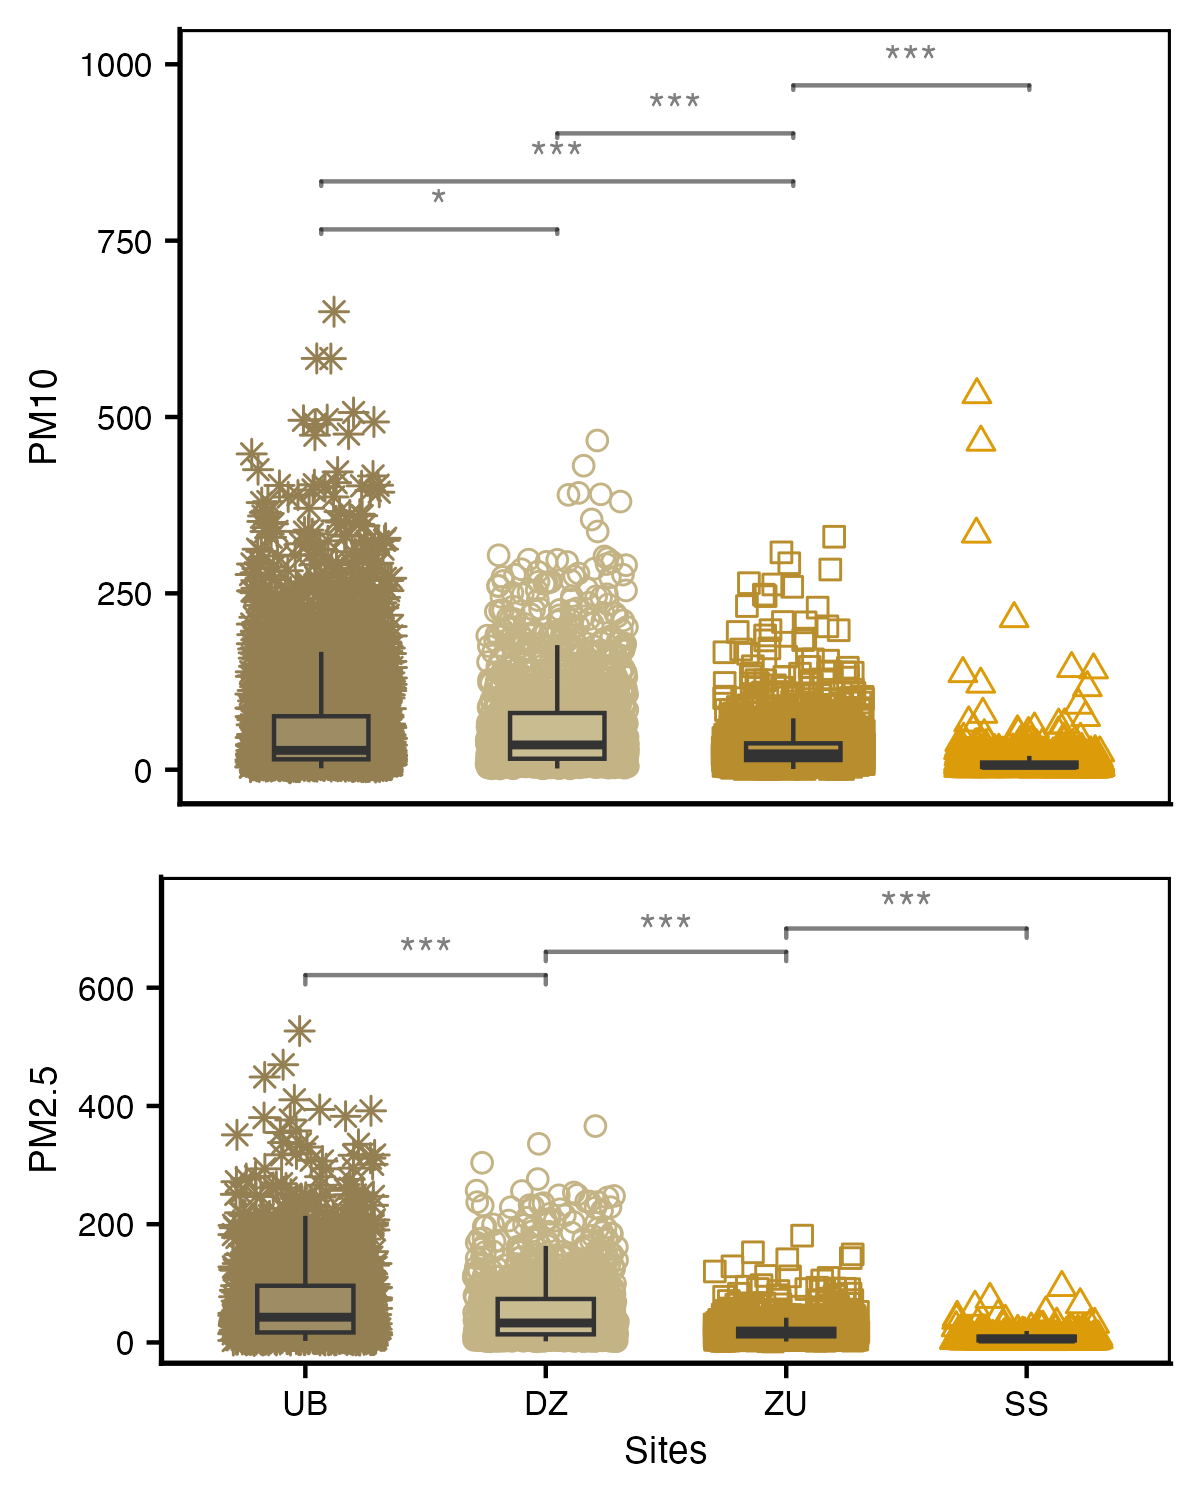
\includegraphics[width=3.125in,height=\textheight,keepaspectratio]{images/figure_3.png}
\caption{Distinct concentrations of coarse and fine particulates among
sites}
\end{figure}

\begin{enumerate}
\def\labelenumi{\arabic{enumi}.}
\tightlist
\item
  Compare the concentrations of PMs at UB is the 2. Significance level
  difference 3. Conclude
\end{enumerate}

\newpage

\begin{figure}
\centering
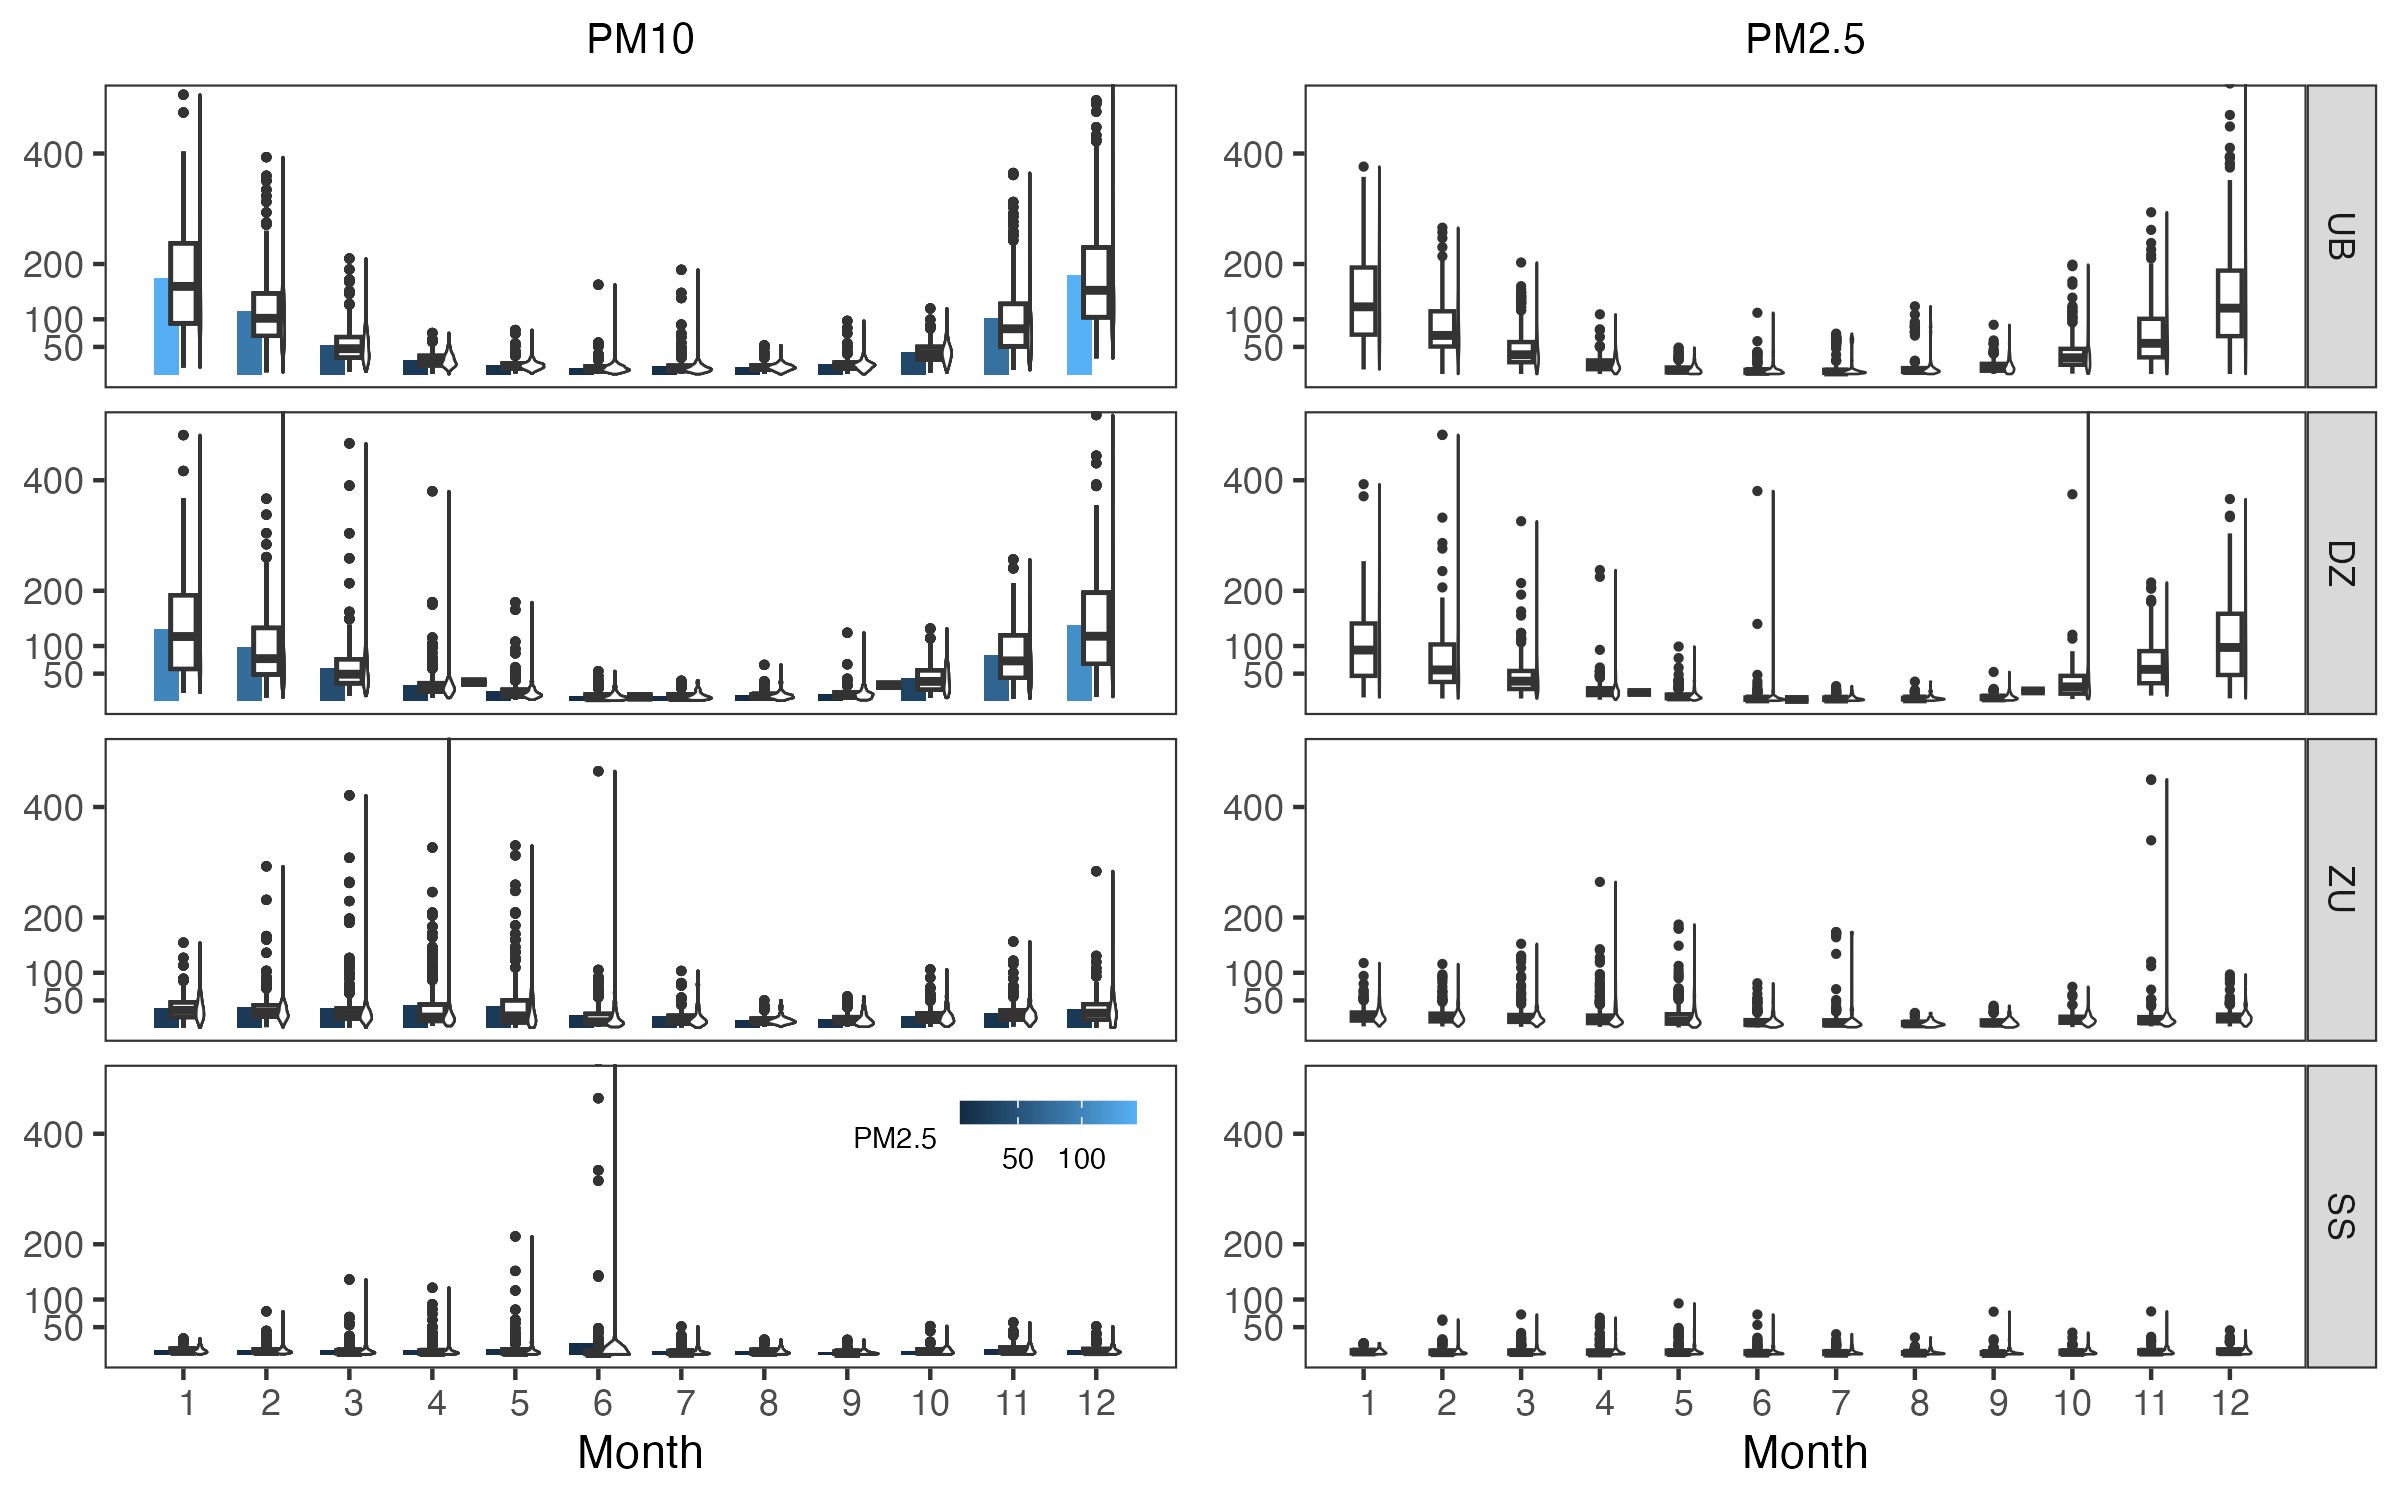
\includegraphics[width=3.4375in,height=\textheight,keepaspectratio]{images/figure_4.png}
\caption{Annual variations of \$PM\_\{10\}\$ and \$PM\_\{2.5\}\$}
\end{figure}

\begin{enumerate}
\def\labelenumi{\arabic{enumi}.}
\tightlist
\item
  Clear annual variations at UB and DZ from pm2.5 pollutions 2. at ZU,
  and SS has a seasonally peaks episodic spring and late autumn from
  PM10
\end{enumerate}

\newpage

\begin{figure}
\centering
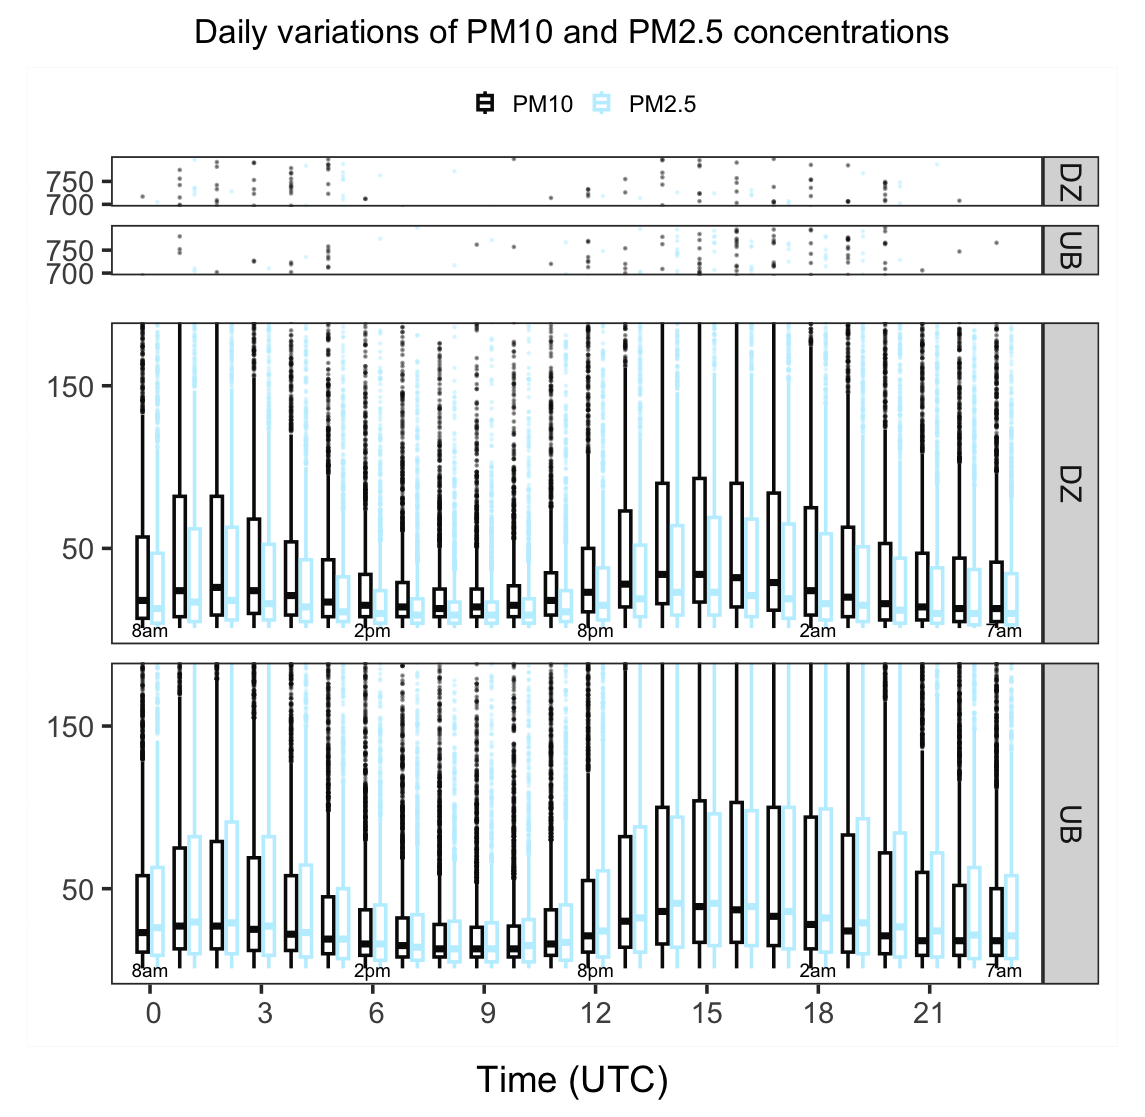
\includegraphics[width=3.125in,height=\textheight,keepaspectratio]{images/figure_5.png}
\caption{Daily variations of \(PM_{10}\) and \(PM_{2.5}\) at UB and DZ
sites}
\end{figure}

\newpage
\subsection{Meteorological influence on $PM_{10}$ and $PM_{2.5}$ variations}
\label{subsec2}

\begin{figure}
\centering
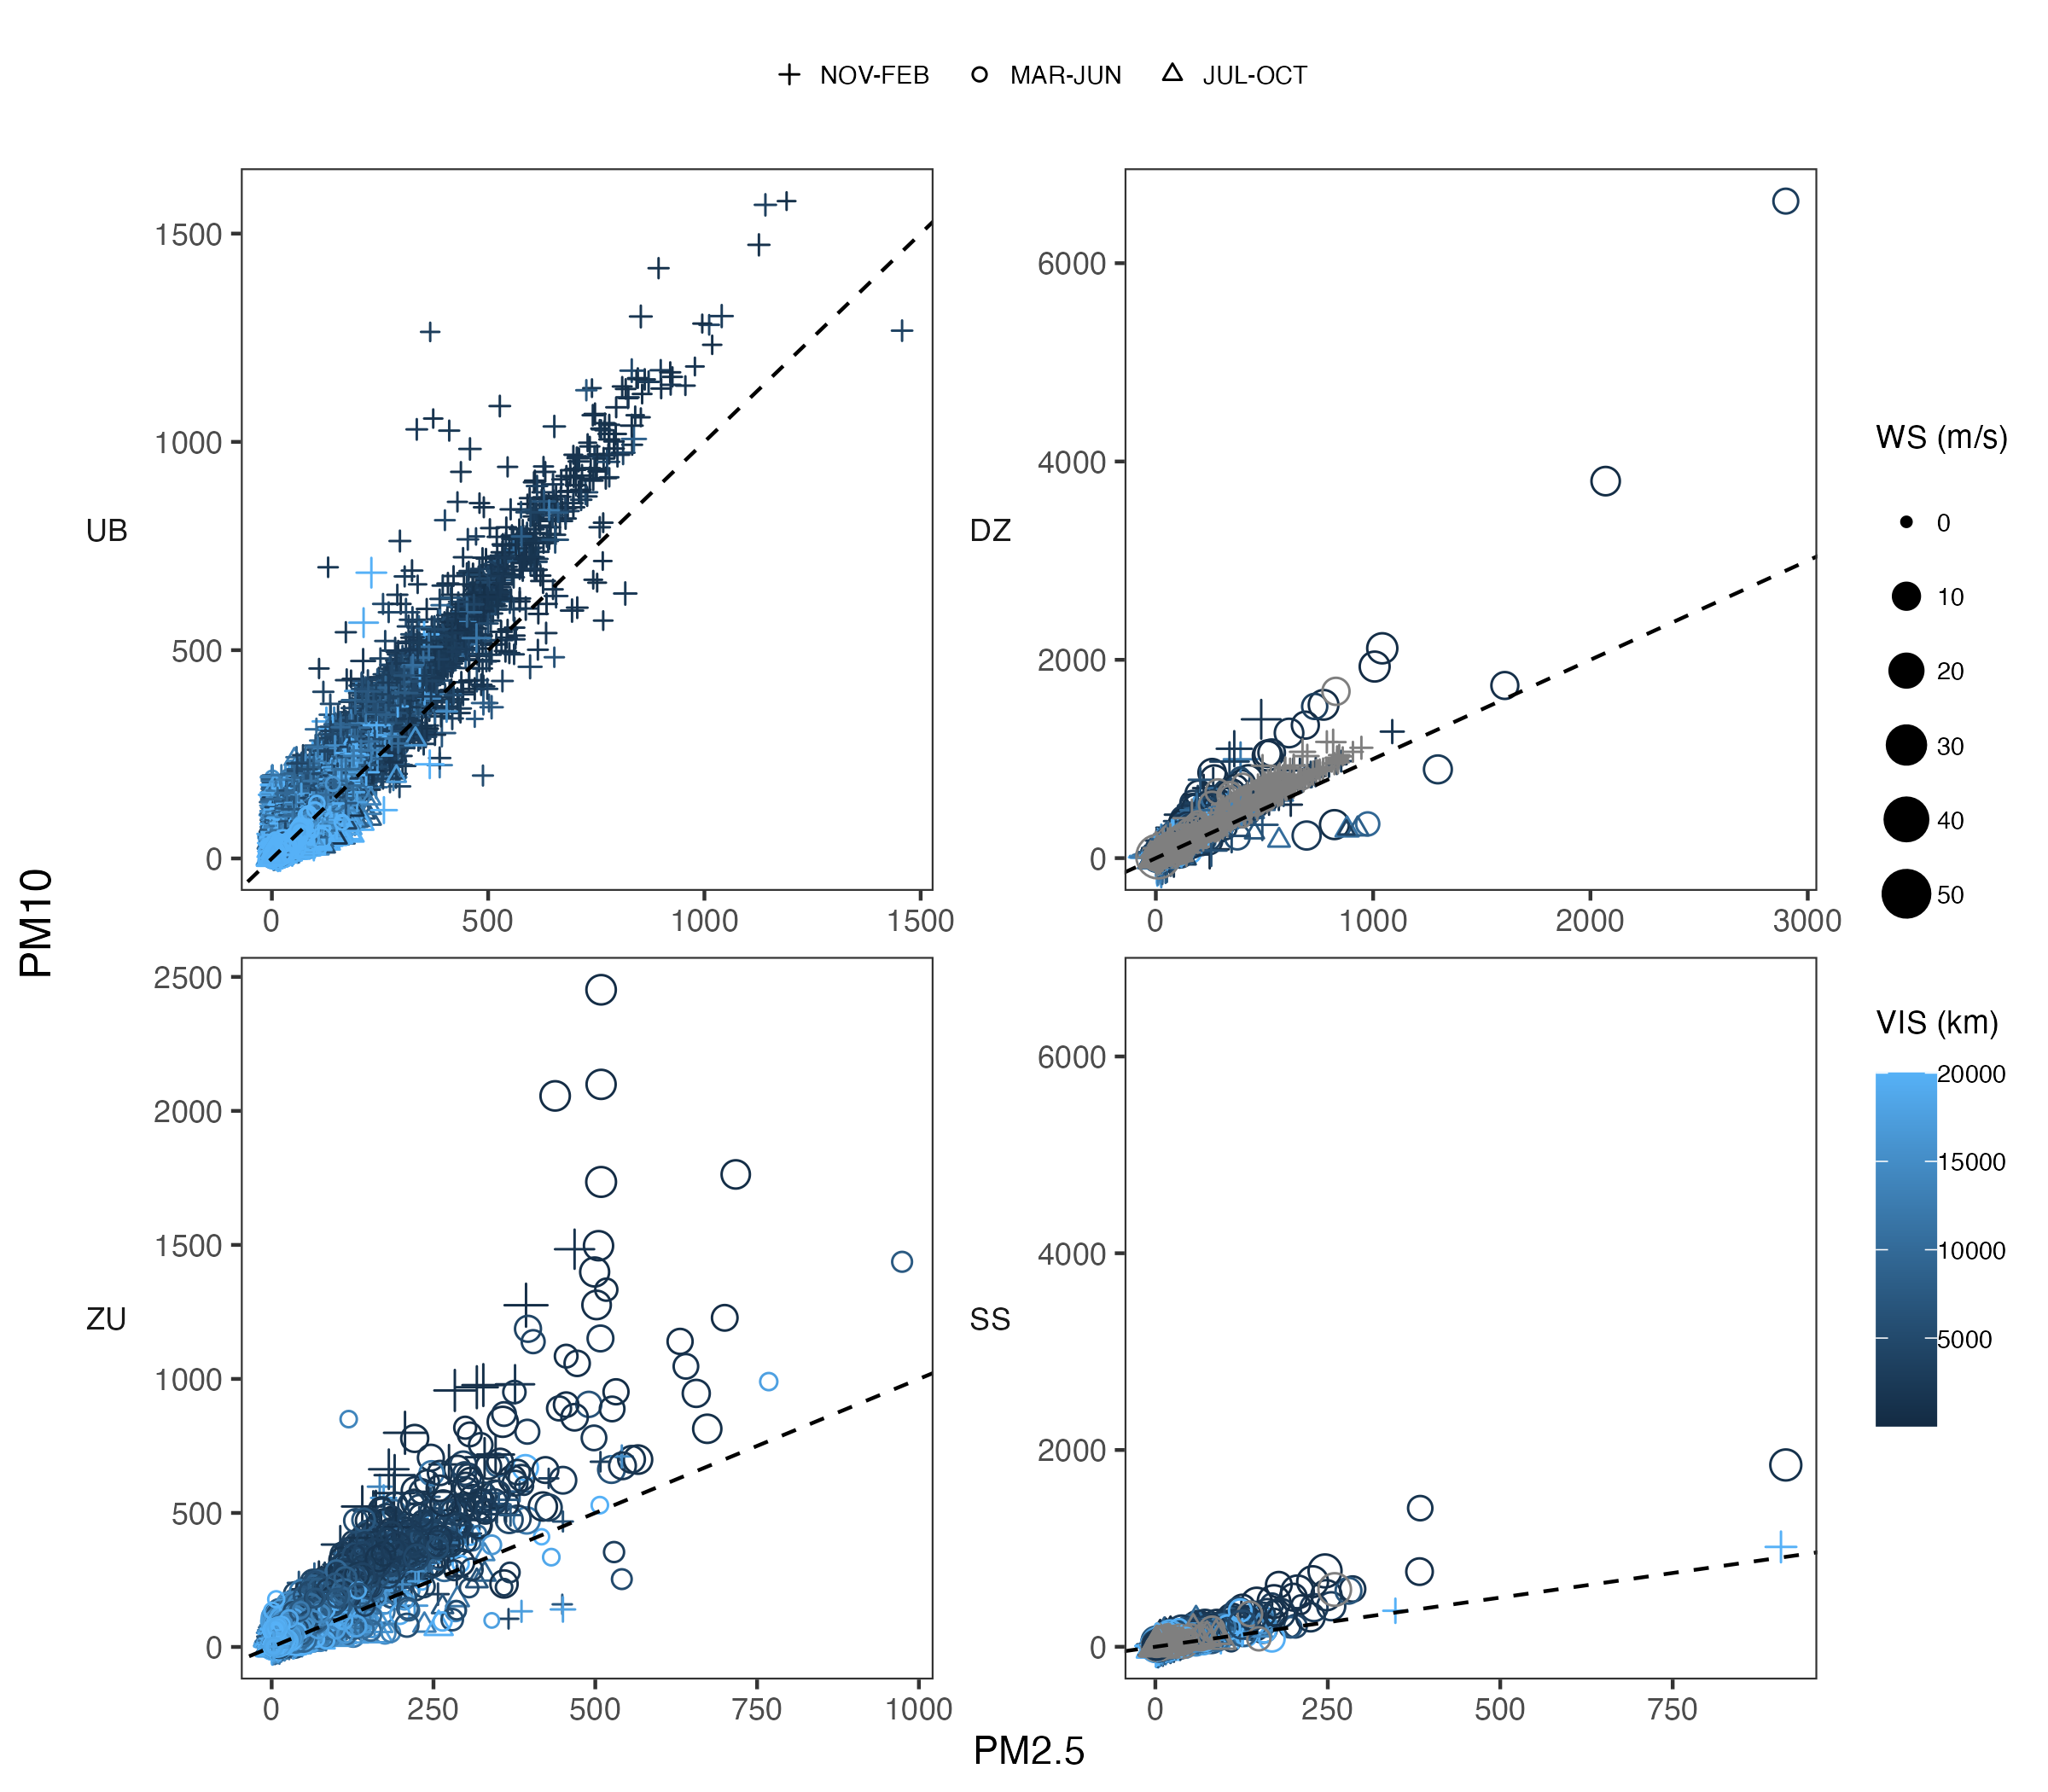
\includegraphics[width=3.125in,height=\textheight,keepaspectratio]{images/figure_6.png}
\caption{Relationships between meteorological major factors and
variations of \(PM_{10}\) and \(PM_{2.5}\)}
\end{figure}

\newpage

\begin{figure}
\centering
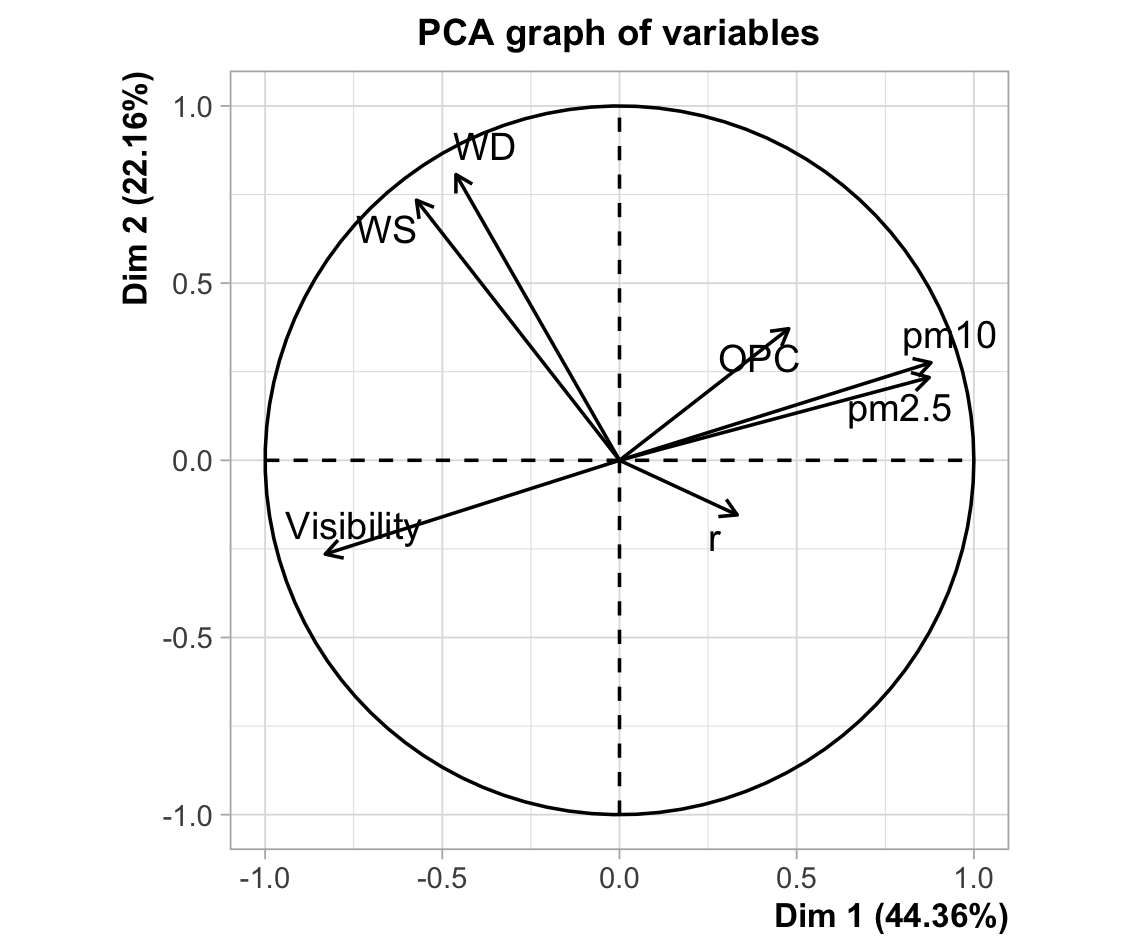
\includegraphics[width=2.08333in,height=\textheight,keepaspectratio]{images/figure_7.png}
\caption{Spatio-temporal distinct feature of variations of \(PM_{10}\)
and \(PM_{2.5}\) with PCA analysis}
\end{figure}

\begin{figure}
\centering
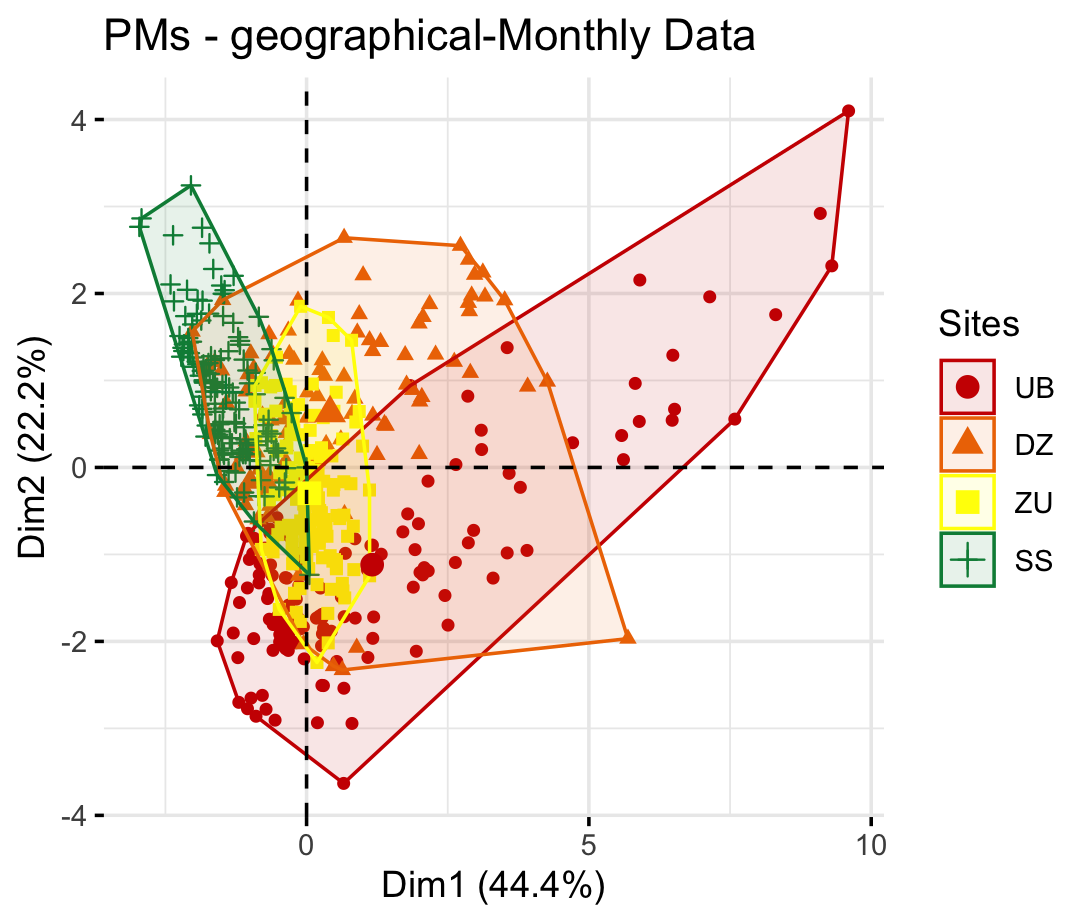
\includegraphics[width=2.08333in,height=\textheight,keepaspectratio]{images/figure_7b.png}
\caption{Patterns of meteorology and PMs at the 4 sites}
\end{figure}

\newpage
\subsection{Trends}

\begin{figure}
\centering
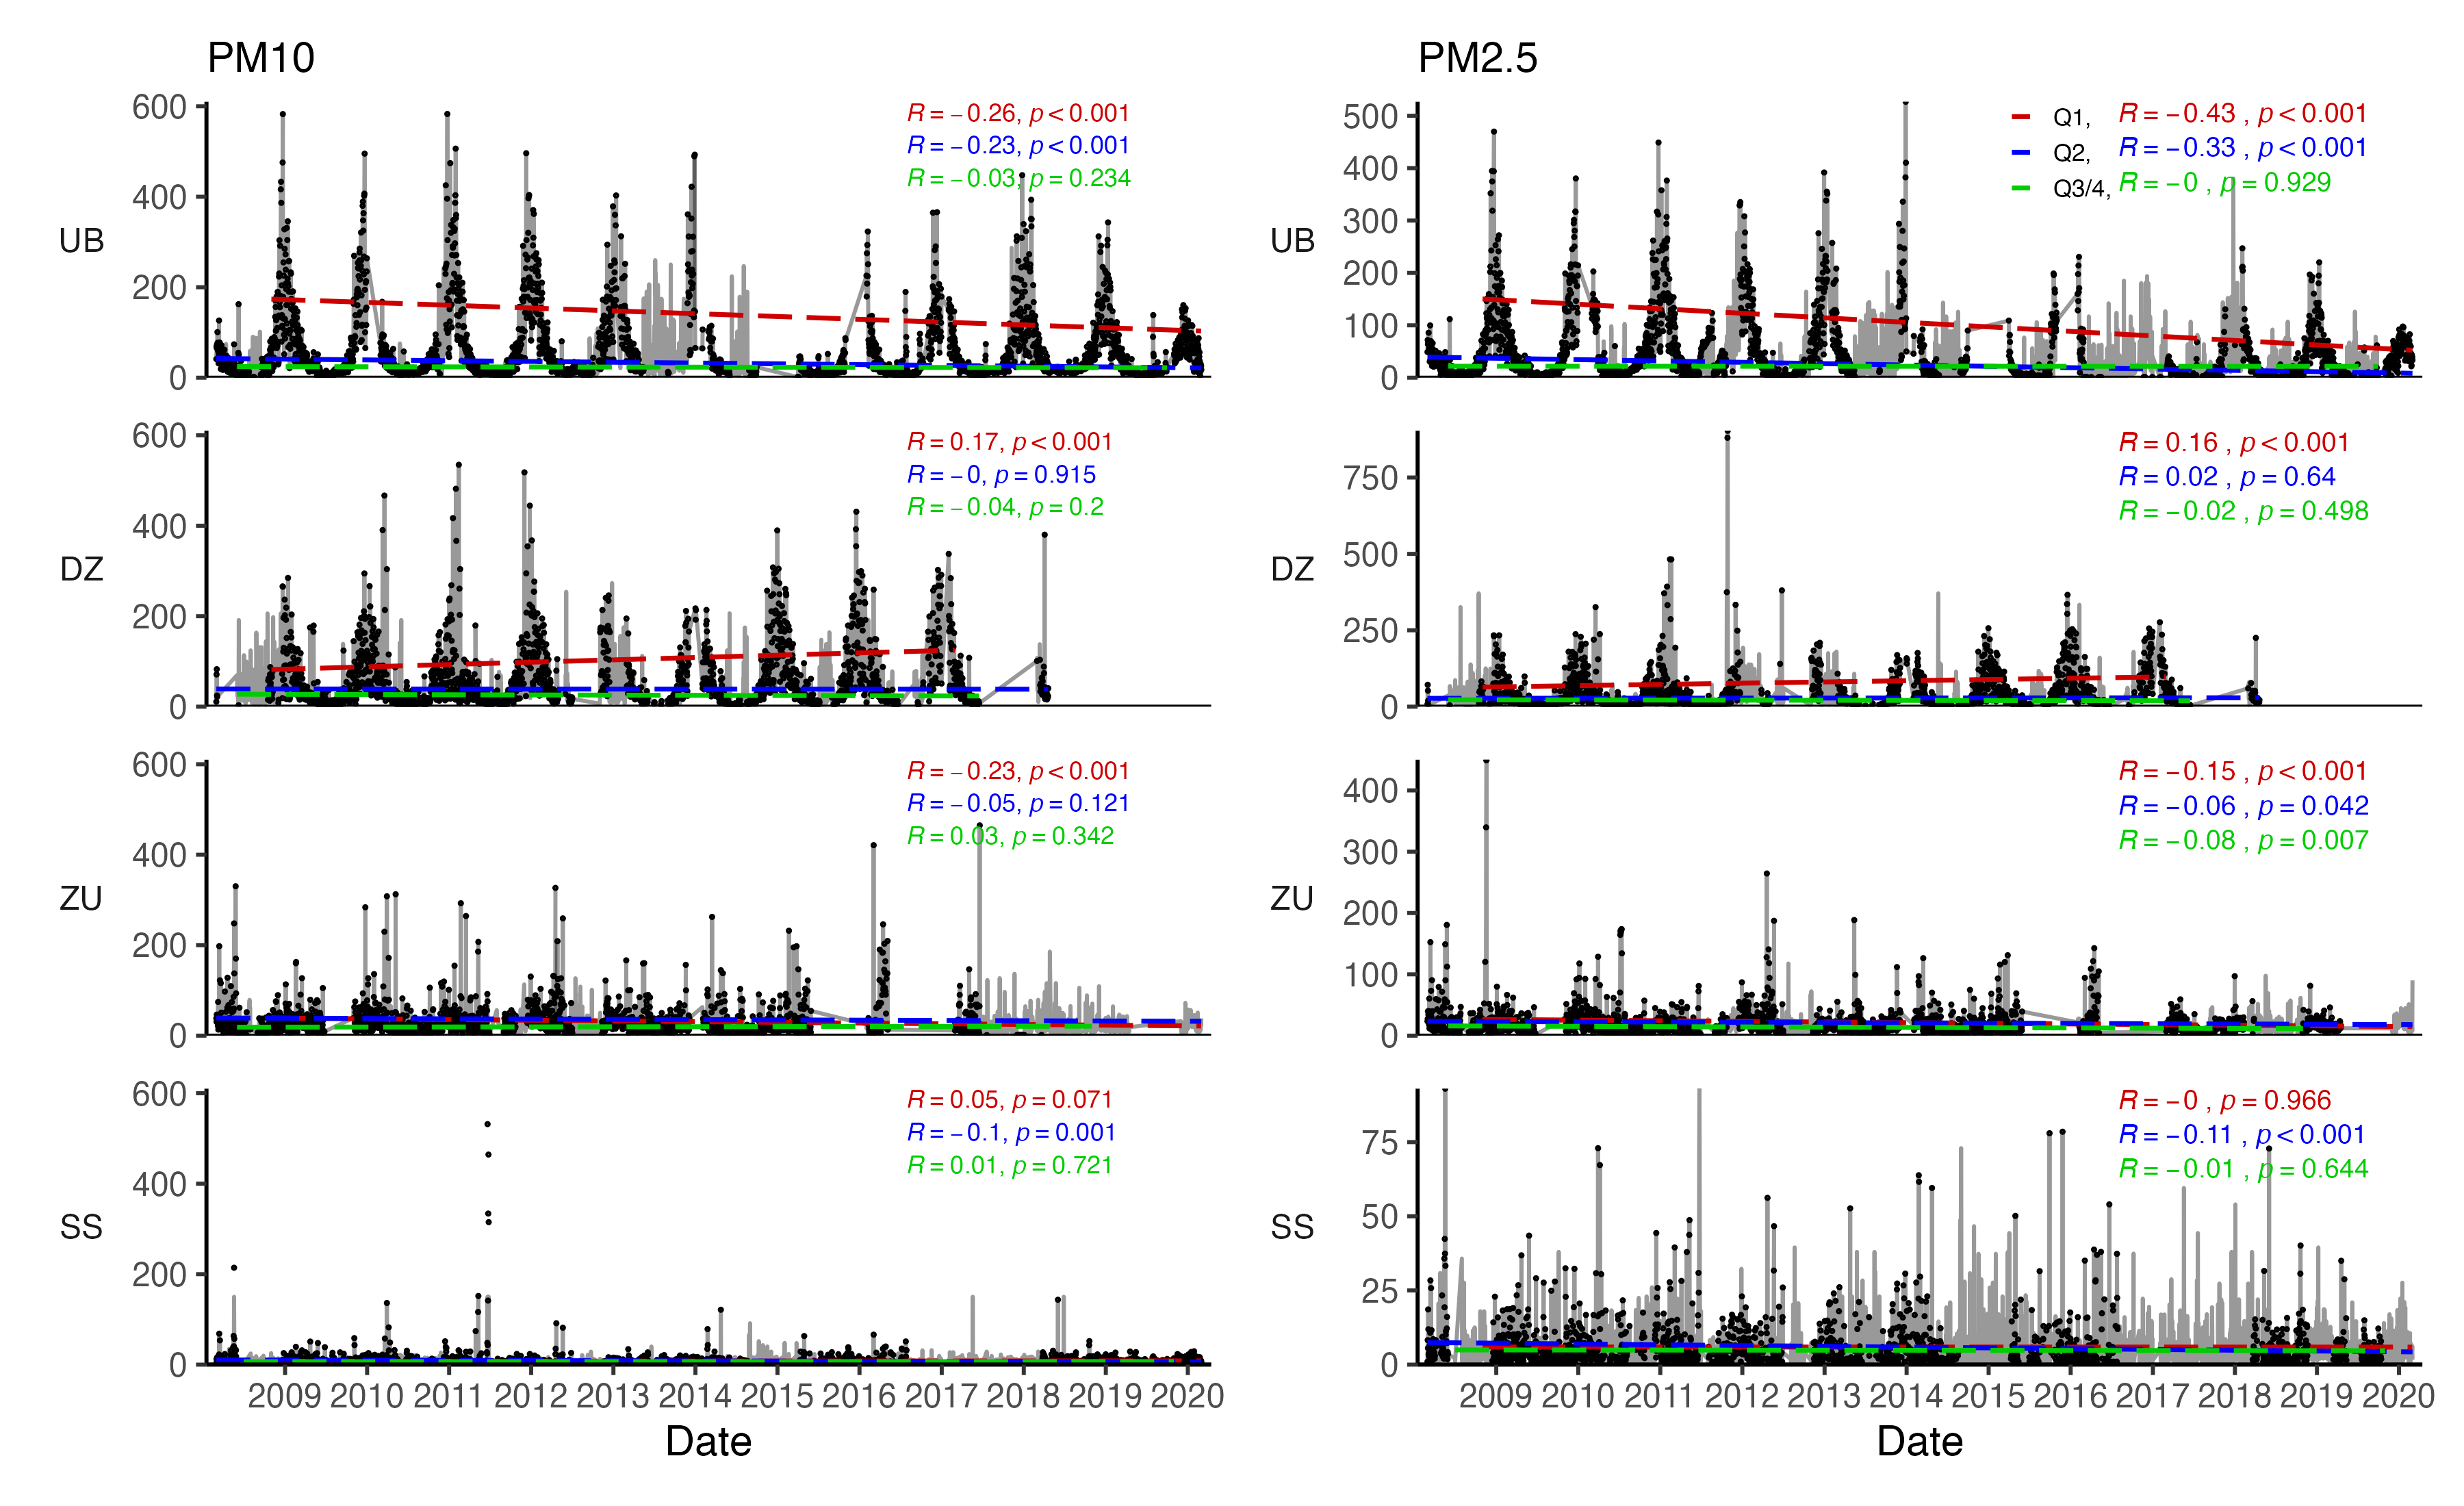
\includegraphics[width=3.125in,height=\textheight,keepaspectratio]{images/figure_8.png}
\caption{Interannual and seasonal trends of \(PM_{10}\) and \(PM_{2.5}\)
variations}
\end{figure}

\newpage

\subsection{Conclusions}\label{conclusions-1}

In this study, we investigated the temporal variations of PM2.5 and PM10
concentrations at the 4 sites of rural and urban those located along the
the wind corridor. Three distinct variations has been detected.

\begin{enumerate}
    \item Air quality in urban sites is episodically dictated by dust events in spring or late autumn, yet seasonally governed by anthropogenic emissions in winter.
    \item Air quality in rural sites of SS and ZU is episodically dictated by dust events in spring or late autumn.
    \item Air quality in rural sites of SS and ZU is episodically dictated by dust events in spring or late autumn.
\end{enumerate}

A clear seasonal variations in the sites of UB and DZ is {[}Air quality
is governed by natural dust emission, and anthropogenic emissions{]} *
Due to rapid increase in urban, and combustion of coal/oyutolgoi for
heating winter conditions results a highly increase in not only capital
city but also towns * In a result, spring coarse dust, plus winter fine
pollutants {[}spring coarse dust is immediately transported and
deposited in the source area, whereas winter fine pollutants is
permanently stayed in the source area due to stagnant atmosphere govern
over entire country., perhaps float- ing in the near surface, deposits
in the surface{]} * Alarms, the Mongolian dust in the spring, optical
properties will be shifted; this gives \ldots{} Gobi dust and sand
storms has become tuiren, from the shoroon shuurga. which clearly
requires the attention.

Following problems

\begin{itemize}
\tightlist
\item
  On downwind regions
\item
  On national-level Demonstrating temporal and spatial variations of air
  particulate matter has become important for understanding
  characteristics of particulate matter in the climate system, providing
  valuable information for well-established air quality measures, and
  illustrating the good trace data for health studies. Because
  particulate pollutants have a great impact on human health (Dockery
  and Pope,1994; Harrison and Yin, 2000; Hong et al., 2002), high
  atmospheric concentrations of these pollutants was a major concern
  particularly in urban areas, in the last 2-3 decades. Recent studies
  highlight that even low concentrations of these pollutants can lead to
  various health issues, and may associate with morbidity and mortality
  across the life span (Zigler et al., 2017). Children exposed to high
  levels of air pollution show increased rates of asthma, decreased lung
  function growth, and increased risk of early markers of cardiovascular
  disease (Bourdrel et al., 2017; Gauderman et al., 2015; Hehua et al.,
  2017). Short-term exposure with high level of PM10 resulted the
  chronic cardiovascular disease in Mongolia (Enkhjargal 2020). In
  addition to these health issues, (prenatal) neurodevelopmental impacts
  such as effects on intelligence, attention, autism, and mood, while
  aging populations experience accelerated cognitive decline when
  exposed to high levels of pollution is detected (Power et al., 2016).
  Long-term exposure to low levels of particulate matter, such as
  concentrations as low as 10 \(\mu g m^{-3}\) (equilibrium to WHO Air
  Quality Guidelines), has been linked to increased lung cancer in the
  EU (Hvidtfeldt et al. 2021), with similar evidences reported in Canada
  (Bai et al., 2019), and significantly higher rates captured in China
  with concentrations up to 30 \(\mu g m^{-3}\). Apparently, pollutants
  of particulate matters has effects to various health issues with the
  different thresholds and exposure durations. However, more in-depth
  and diversified research on air pollution and its health effects is
  essential, with the detailed information is necessary (Tan et al

  \begin{enumerate}
  \def\labelenumi{\arabic{enumi})}
  \setcounter{enumi}{2020}
  \tightlist
  \item
    to have accuracy of assessing exposure to air pollution during
    developmentally relevant time periods, such as trimesters or months
    (Becerra et al., 2013; Gong et al., 2014; Kalkbrenner et al., 2014)
    or weeks (Chiu et al., 2016). Many research findings/Numerous
    research findings have advanced the field, and air quality indices
    is widely used for providing guidance, and public perception of air
    quality has been improved (Mirabelli et al., 2020).
  \end{enumerate}
\end{itemize}

\newpage

\subsection{Materials and Methods}\label{materials-and-methods}

\subsubsection{Materials}\label{materials}

\subsubsection{Methods 3,000 words}\label{methods-3000-words}

\subsection{Acknowledgements}\label{acknowledgements}

Keep acknowledgements brief and do not include thanks to anonymous
referees or editors, or effusive comments. Grant or contribution numbers
may be acknowledged.

\subsection{Figures (10)}\label{figures-10}

Figure legends should be \textless350 words each. They should begin with
a brief title sentence for the whole figure and continue with a short
statement of what is depicted in the figure, not the results (or data)
of the experiment or the methods used. Legends should be detailed enough
so that each figure and caption can, as far as possible, be understood
in isolation from the main text.

Tables. Each table should be prepared using the Table menu in Word or
the table environment in TeX/LaTeX and accompanied by a short title
sentence describing what the table shows. Further details can be
included as footnotes to the table.

\subsection{References (70)}\label{references-70}

\subsection{Supplementary}\label{supplementary}

Author contributions. You must include a statement that specifies the
individual contributions of each co-author. For example: ``A.P.M.
`contributed' Y and Z; B.T.R. `contributed' Y,'' etc. See our authorship
policies for more details.

Competing interests. Submission of a competing interests statement is
required for all content of the journal.

Materials \& Correspondence. Indicate the author(s) to whom
correspondence and material requests should be addressed.

Supplementary information Please submit supplementary figures, small
tables and text as a single combined PDF document. Tables longer than
one page should be provided as an Excel or similar file type. For
optimal quality video files please use H.264 encoding, the standard
aspect ratio of 16:9 (4:3 is second best) and do not compress the video.
We encourage submission of step-by-step synthesis procedures for
chemical compounds and data on compound characterization. Supplementary
information is not copyedited, so please ensure that it is clearly and
succinctly presented, and that the style and terminology conform to the
rest of the manuscript.

\subsection{Materials and Methods}\label{materials-and-methods-1}

\subsubsection{A description of study
sites}\label{a-description-of-study-sites}

According to the spatial magnitude of wind stress in Mongolia (Figure
1), the largest magnitude of wind speed is on the Gobi sites,
particularly those located in the southeast edge of the country.

\begin{itemize}
\tightlist
\item
  The impact of high winds on plant diversity varies across
  environmental gradients of precipitation and soil fertility (Milchunas
  et al., 1988).
\item
  In the desert steppe zone, species richness was lower in the drier
  years but did not vary with grazing pressure.
\item
  In the steppe zone, species richness varied significantly with grazing
  pressure but did not vary between years. Species richness is not
  impacted by grazing gradient in desert steppe, but it is in the steppe
  (Cheng et al., 2011).
\end{itemize}

In the last 2 decades, due to poverty and natural disasters there is
population immigration has taken place from the rural to urban,
especially to capital city of Mongolia. Due to tiny infrastructure to
provide the mega city with the dense population, it introduces the urban
pollution. Therefore, Ulaanbaatar air particulate matter mainly reflects
the coal burning, and partly, natural dust.

Consequently, the atmospheric environment and climate for Mongolian Gobi
has been impacted the most by frequent dust and and sand storm in the
spring.

Our study was carried out in Dalanzadgad (town center) (Tbl. 1; 43.57°N,
104.42°E), Sainshand (Tbl. 1; 44.87°N, 110.12°E) and Zamyn-Uud (Tbl. 1;
43.72°N, 111.90°E) in the Gobi Desert, and at Ulaanbaatar (Tbl.??.??°N,
104.42°E) (city center) located in the temperate Mongolian steppe of
Mongolia (Figure 2). Nomads and settlements of this sum have raised a
large number of livestock, and they rank at number 30 out of 329 sums
for the largest number of livestock raised per sum (Saizen et al.,
2010). In the last decade, the number of dust events associated with
wind erodibility increased by 30 \% in Bayan-Önjüül (Kurosaki et al.,
2011). This is an area where dust emissions activity has been monitored
on a long-term basis (Shinoda et al., 2010a) at a dust observation site
(DOS) adjacent to the study site (Fig. 1a). According to long-term
meteorological observations made at the monitoring station of the
Institute of Meteorology and Hydrology of Mongolia located near the
site, the prevailing wind direction is northwest. Mean annual
precipitation is 163 mm, and mean temperature is 0.1◦C for the period
1995 to 2005 (Shinoda et al., 2010b). Soil texture is dominated by sand
(98.1 \%, with only 1.3 \% clay and 0.6 \% silt; Table 1; Shinoda et
al., 2010a). Insert figure legends with the first sentence in bold, for
example:

\newpage

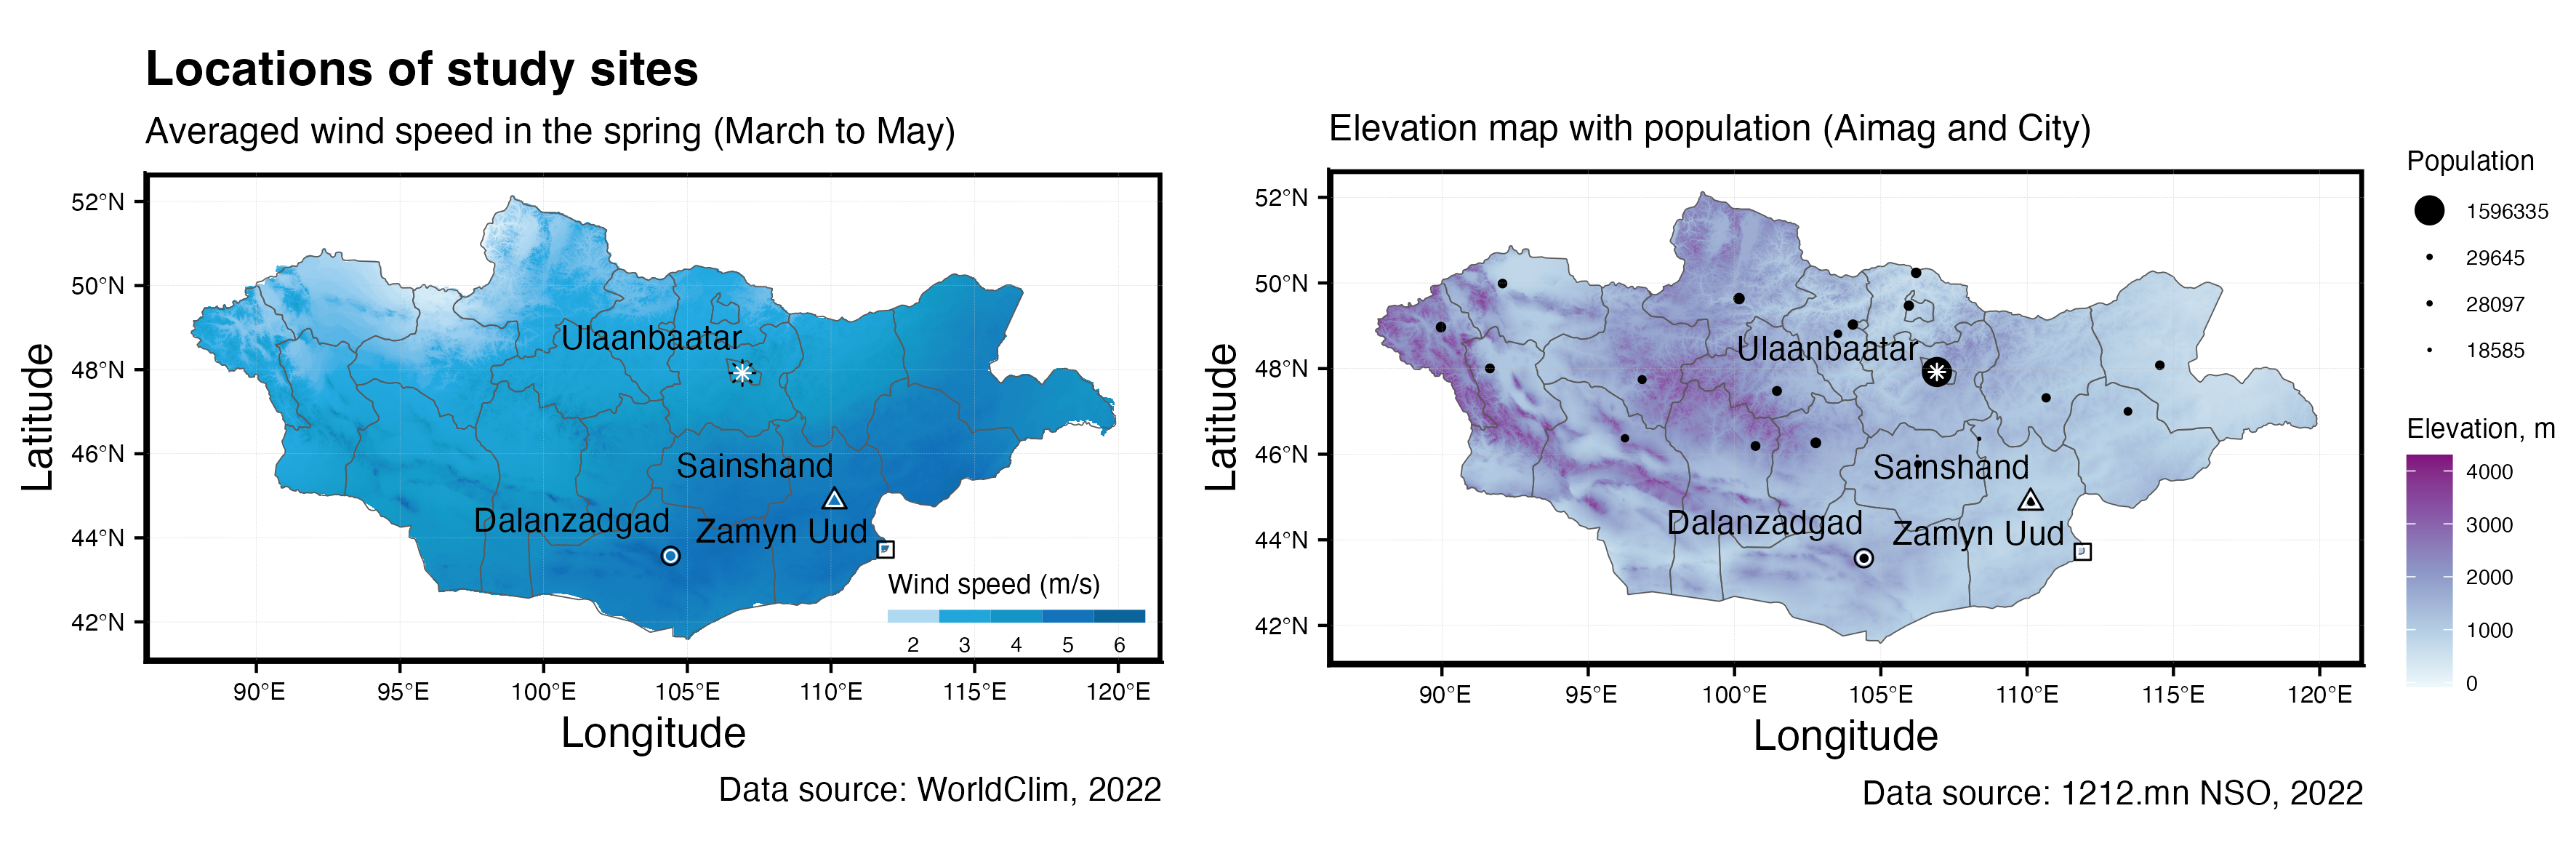
\includegraphics[width=3.125in,height=\textheight,keepaspectratio]{images/figure_1.png}{]}

\begin{figure}
\centering
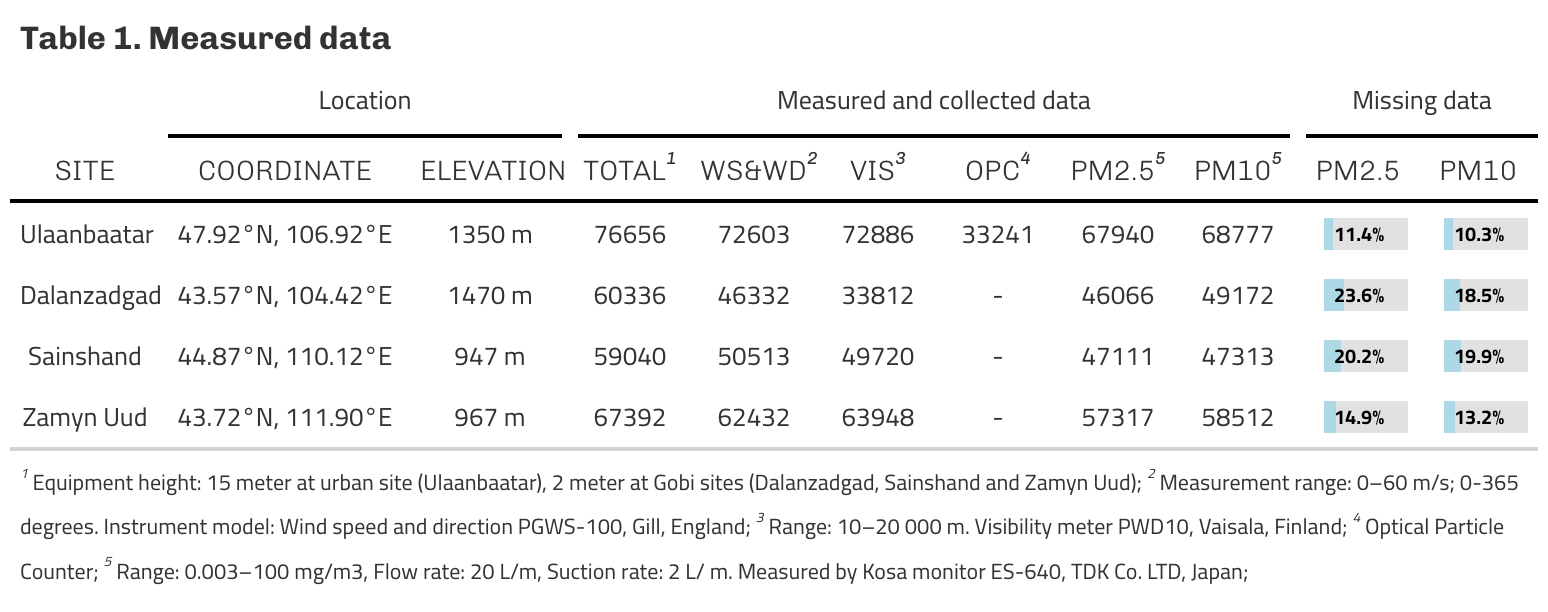
\includegraphics[width=4.16667in,height=\textheight,keepaspectratio]{images/table_1.png}
\caption{\textbf{Table 1}. A description of datasets obtained at the
sites}
\end{figure}

\newpage

\begin{figure}
\centering
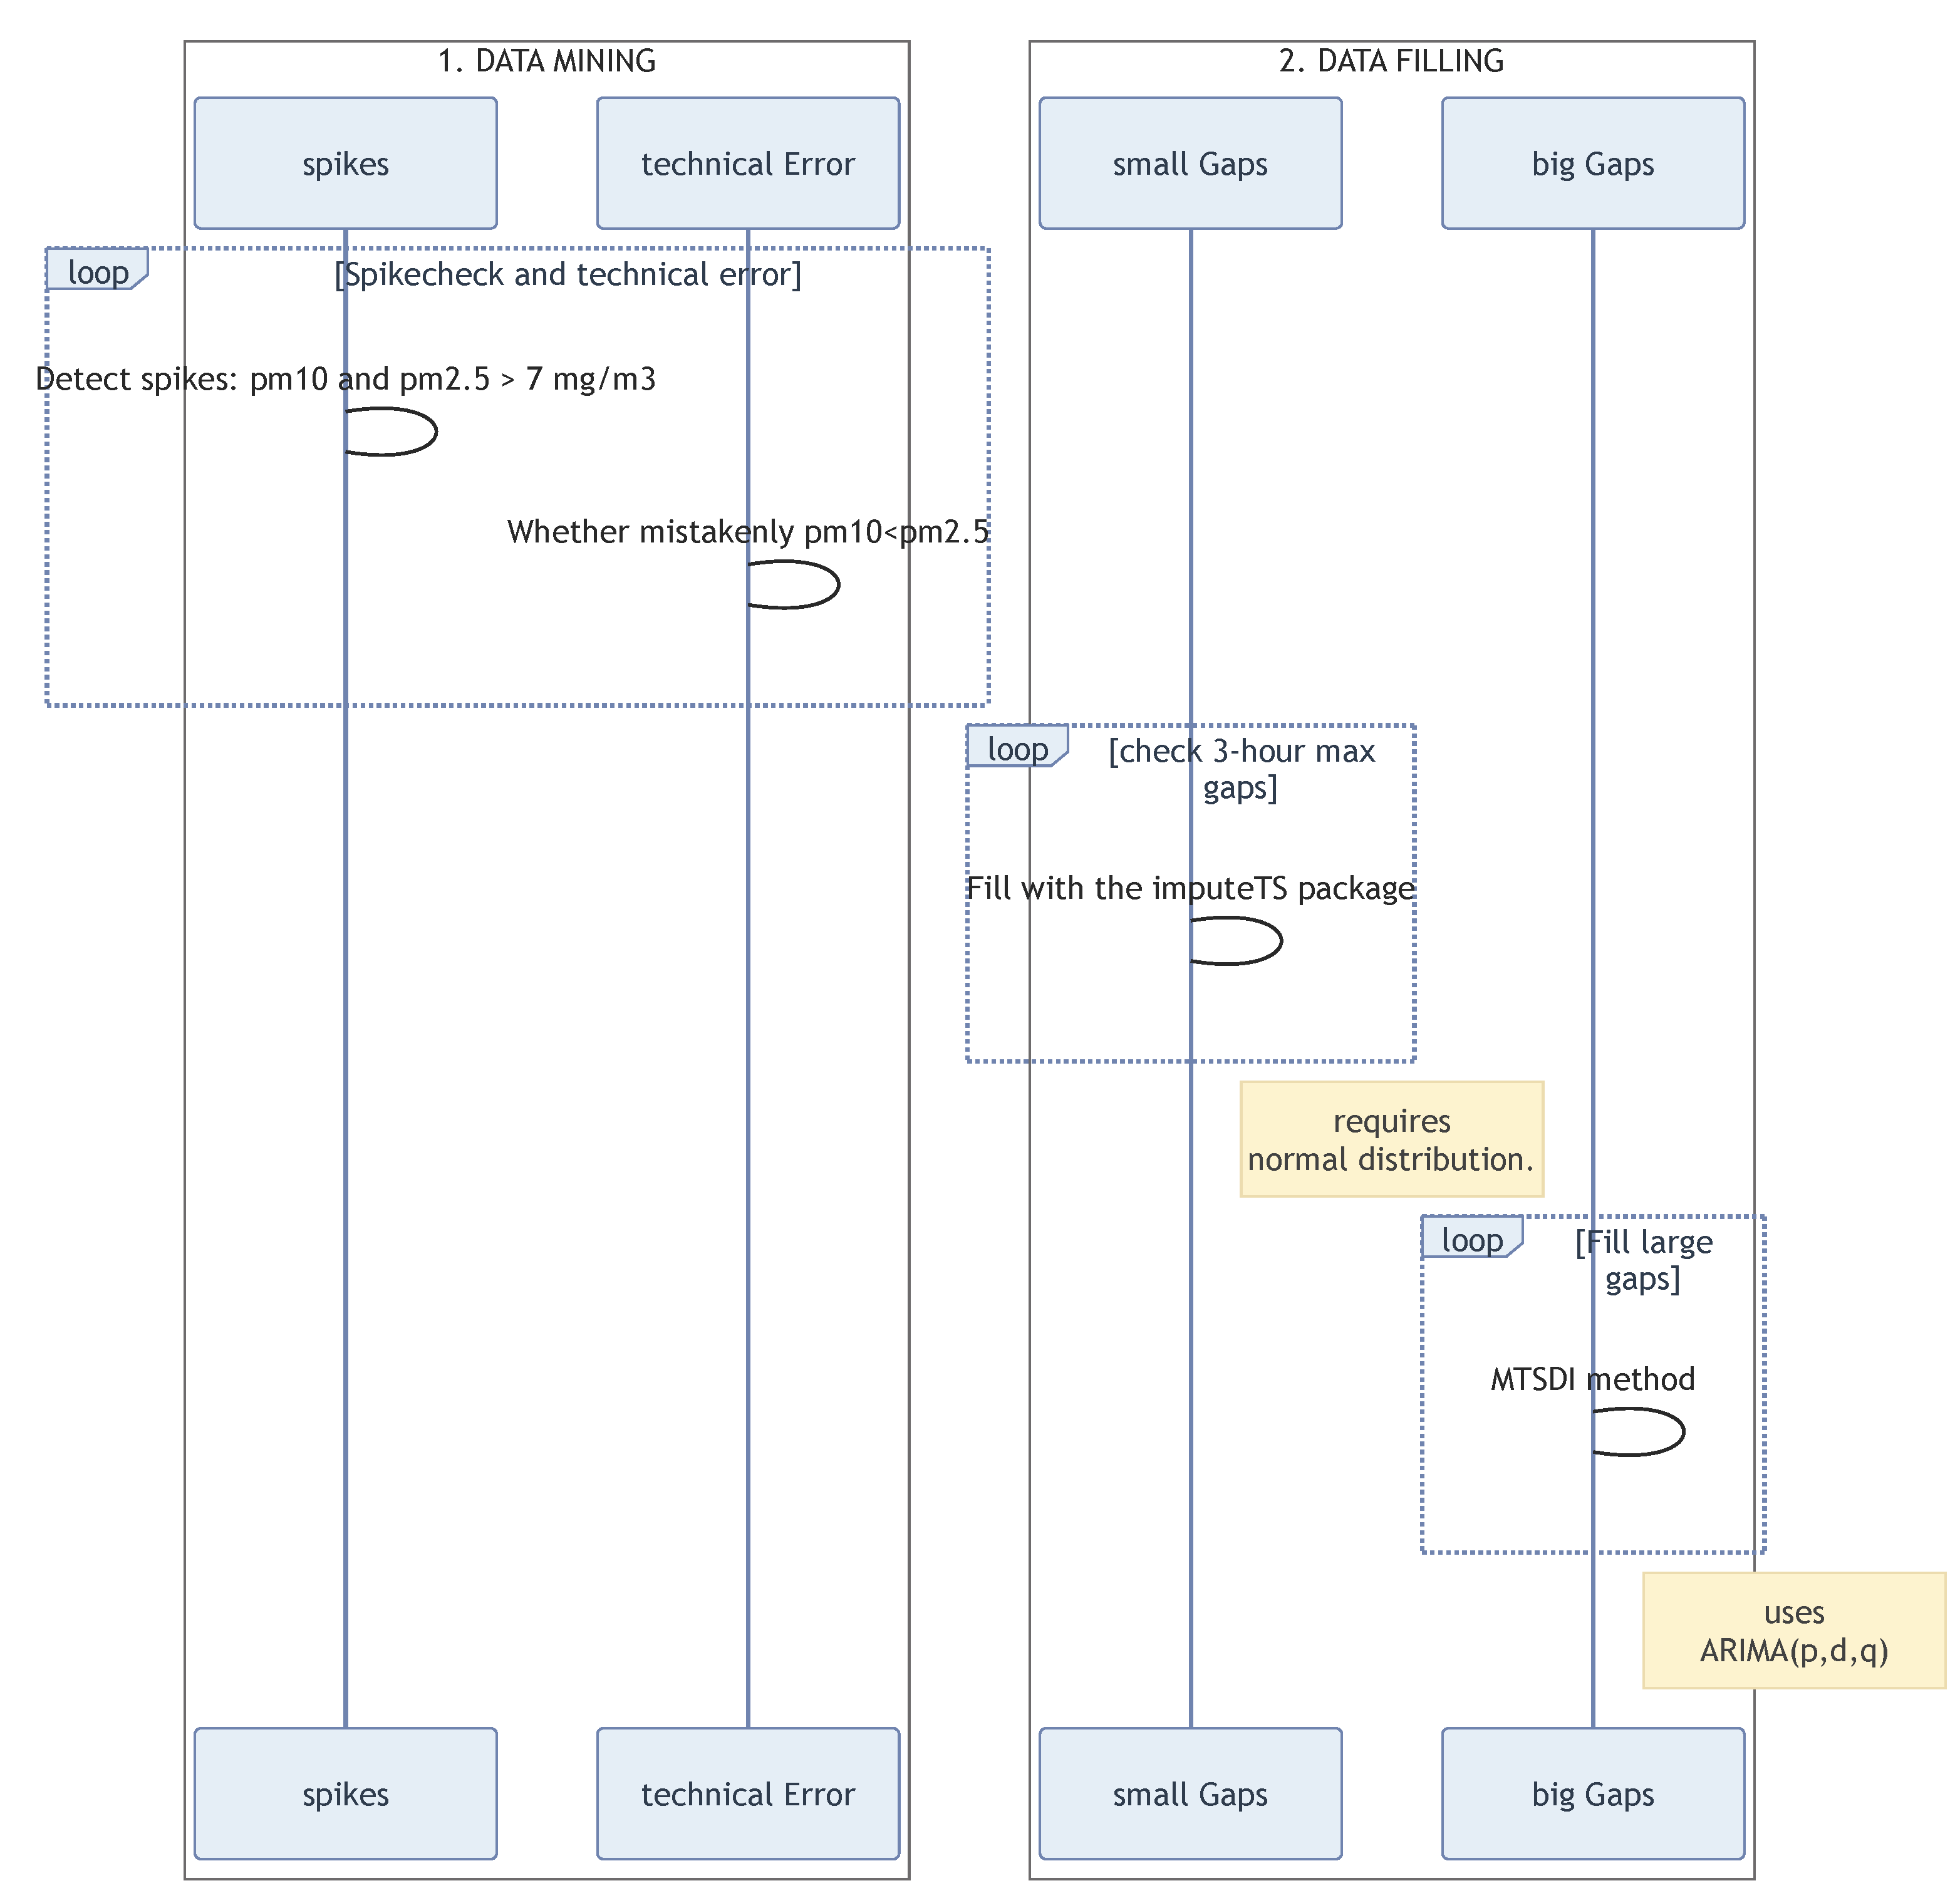
\includegraphics[width=3.125in,height=\textheight,keepaspectratio]{images/scheme_1.png}
\caption{Scheme 1. Data handling procedure}
\end{figure}

\newpage

\begin{figure}
\centering
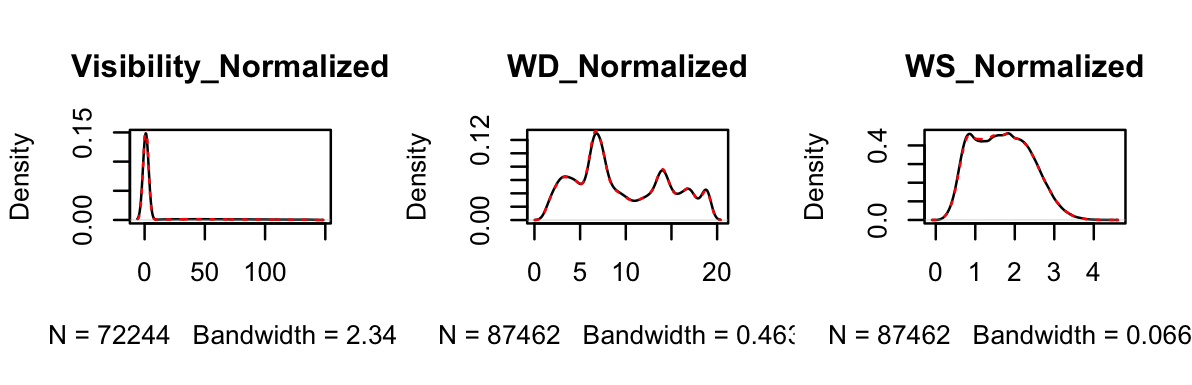
\includegraphics[width=3.125in,height=\textheight,keepaspectratio]{images/figure_2b.png}
\caption{Figure 2. Data gap filling}
\end{figure}

\begin{figure}
\centering
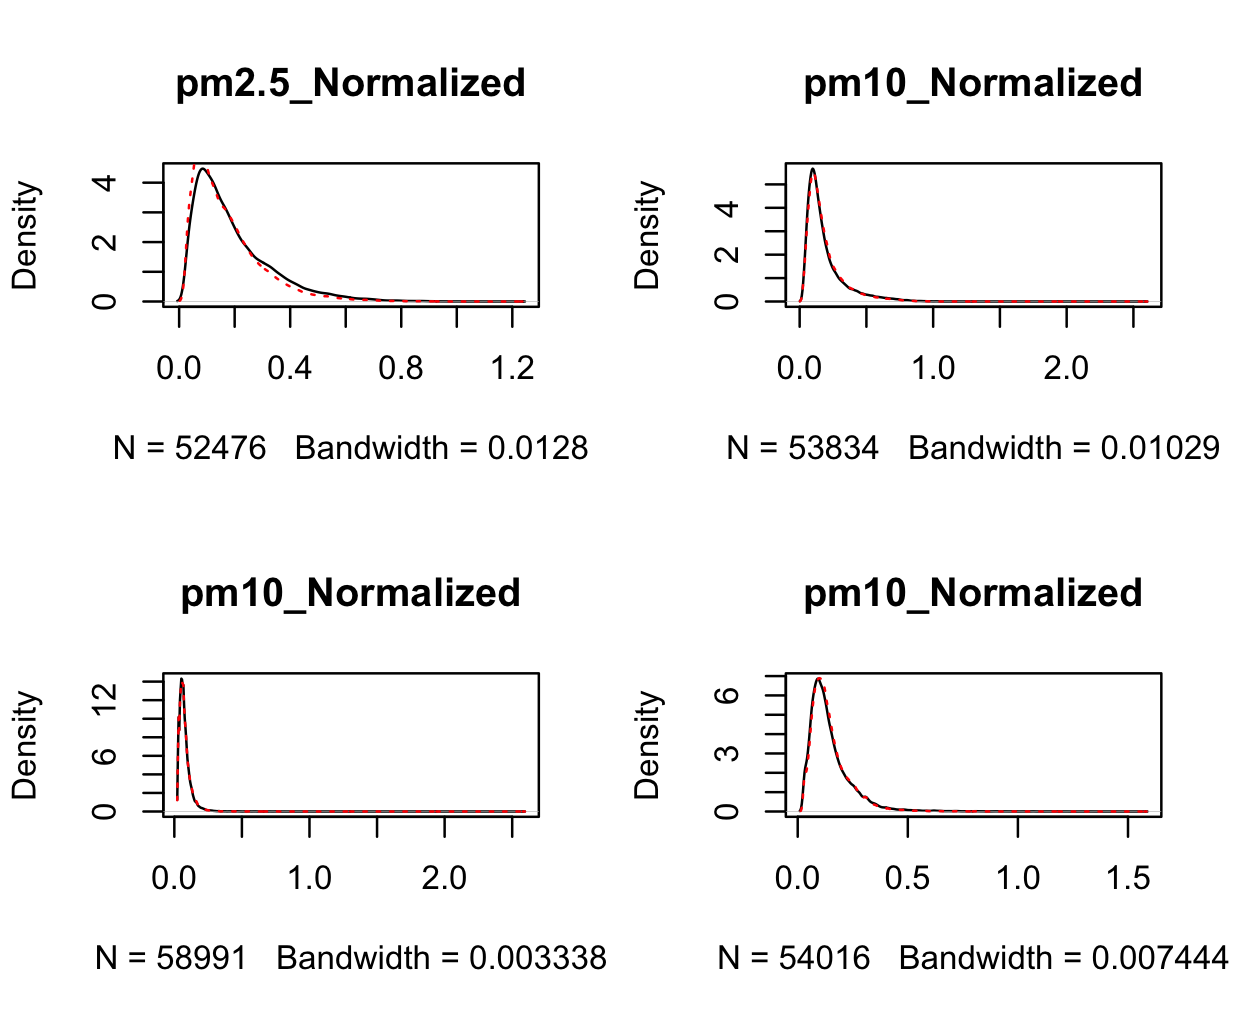
\includegraphics[width=3.125in,height=\textheight,keepaspectratio]{images/figure_2c.png}
\caption{Figure 2b. Data gap filling}
\end{figure}

\newpage

\subsection{References}\label{references}

\end{document}
